\def\us{\char`\_}

\documentclass[a4paper, 12pt]{article}
%\documentclass{article}

\usepackage{fullpage}
\usepackage{pgf}
\usepackage{tikz}
\usetikzlibrary{arrows,automata,shapes}
\usepackage{multirow}
\usepackage{color}
\usepackage[latin1]{inputenc}
\usepackage{verbatim}
\usepackage{amsmath}
\usepackage{textcomp}
\usepackage{times,mathptmx}
\usepackage{chngcntr}
\usepackage{hyperref}
\usepackage{enumitem}
\usepackage{scrextend}
%\usepackage[table]{xcolor}
\usepackage{listings}
\definecolor{light-gray}{gray}{0.95}
%\usepackage[firstpage]{draftwatermark}

% for glossary
% nopostdot - no dot at the end of index entires
\usepackage[nogroupskip,nopostdot,counter=subsubsection]{glossaries}
\renewcommand{\glossarysection}[2][]{}
\usepackage{listings}
\usepackage{cancel}
\graphicspath{ {../../../../figures/} }

\newenvironment{packed_enum}{
\begin{enumerate}[leftmargin=0pt,topsep=-12pt]
	\setlength{\itemsep}{1pt}
	\setlength{\parskip}{0pt}
	\setlength{\parsep}{0pt}
}{\end{enumerate}}

\newenvironment{packed_items}{
\begin{itemize}[topsep=-12pt]
	\setlength{\itemsep}{1pt}
	\setlength{\parskip}{0pt}
	\setlength{\parsep}{0pt}
}{\end{itemize}}

%  \begin{itemize}[leftmargin=50pt] %,topsep=-12pt]
\newenvironment{packed_items_snmp_obj}{
  \begin{itemize}[leftmargin=50pt]
	\setlength{\itemsep}{1pt}
	\setlength{\parskip}{0pt}
	\setlength{\parsep}{0pt}
  \renewcommand\labelitemi{--}
}{\end{itemize}}

\newenvironment{pck_descr}{
\begin{itemize}[leftmargin=0pt,topsep=-12pt]
	\setlength{\itemsep}{1pt}
	\setlength{\parskip}{0pt}
	\setlength{\parsep}{0pt}
}{\end{itemize}}

\newenvironment{pck_proc}{
\begin{enumerate}[leftmargin=15pt,topsep=-12pt]
	\setlength{\itemsep}{1pt}
	\setlength{\parskip}{0pt}
	\setlength{\parsep}{0pt}
}{\end{enumerate}}


%%%%%%%%%%%%%%%%%%%%%%%%%%%%%%%%%%%%%%%%%%%%%%%%%%%%%%%%%%%%%%%%%%%%%%%%%%%
% creating subsubsubsection notation
% src: http://www.latex-community.org/forum/viewtopic.php?f=5&t=791
%%%%%%%%%%%%%%%%%%%%%%%%%%%%%%%%%%%%%%%%%%%%%%%%%%%%%%%%%%%%%%%%%%%%%%%%%%%
\setcounter{secnumdepth}{6}
\renewcommand\theparagraph{\Alph{paragraph}}

\makeatletter
\renewcommand\paragraph{\@startsection{paragraph}{4}{\z@}%
                                     {-3.25ex\@plus -1ex \@minus -.2ex}%
                                     {0.0001pt \@plus .2ex}%
                                     {\normalfont\normalsize\bfseries}}
\renewcommand\subparagraph{\@startsection{subparagraph}{5}{\z@}%
                                     {-3.25ex\@plus -1ex \@minus -.2ex}%
                                     {0.0001pt \@plus .2ex}%
                                     {\normalfont\normalsize\bfseries}}
\counterwithin{paragraph}{subsubsection}
\counterwithin{subparagraph}{paragraph}
\makeatother
%%%%%%%%%%%%%%%%%%%%%%%%%%%%%%%%%%%%%%%%%%%%%%%%%%%%%%%%%%%%%%%%%%%%%%%%%%%%%%%%

\newcommand{\eqoffset}[1]{%
  {\ensuremath{%
      {\text{offset}}_{#1}}%
  }%
}
\newcommand{\eqdelay}[1]{{\text{delay}}_{#1}}
\newcommand{\eqasymm}{{\text{asymmetry}}}

% for glossary, set way of sorting entries
\makenoidxglossaries
% don't bold entries, texttt them
\renewcommand*{\glsnamefont}[1]{\texttt{\textmd{#1}}}

\newglossary*{snmp_status}{SNMP's status objects}
\newglossary*{snmp_expert}{SNMP's expert objects}
\newglossary*{snmp_other}{Objects from other MIBs}
% alphabetical list of all entries
\newglossary*{snmp_all}{All SNMP objects}

\defglsentryfmt[snmp_status]{\texttt{\glsentryfmt}}
\defglsentryfmt[snmp_expert]{\texttt{\glsentryfmt}}
\defglsentryfmt[snmp_other]{\texttt{\glsentryfmt}}
% macro to add entires
\newcommand{\snmpadd}[1]{
  \glspl{#1}\glsadd{x#1}%
}

% helpers to add glossary entries
% add newline to non empty strings. For descriptions.
\newcommand{\descr}[1]{
  \ifx&#1&%
    %
  \else% put fixed space
    \\#1
  \fi
}

% {MIB}{parent}{object}{comment}{glossary_name}
\newcommand{\snmpentry}[5]{%
  \ifx&#2&% if parameter 2 is empty don't add parent
    \newglossaryentry{#1::#3}{%
      type=#5,%
      name={#3},%
      plural={#1::#3},% used to display name not plural
      user1={#1},% MIB
      description={\descr{#4}}%
      }%
  \else
      \newglossaryentry{#1::#3}{%
      type=#5,%
      name={#3},%
      description={\descr{#4}},%
      plural={#1::#3},% used to display name not plural
      user1={#1},% MIB
      parent={#1::#2}%
      }%
  \fi
  % add entry to alphabetical list
  \newglossaryentry{x#1::#3}{%
      type=snmp_all,%
      name={#1::#3},%
      description={}
      }%
}

% {MIB}{parent}{object}{comment}
\newcommand{\snmpentrye}[4]{%
  \snmpentry{#1}{#2}{#3}{#4}{snmp_expert}
}

% {MIB}{parent}{object}{comment}
\newcommand{\snmpentrys}[4]{%
  \snmpentry{#1}{#2}{#3}{#4}{snmp_status}
}

% command to add snmp objects from other MIBs
% {MIB}{parent}{object}{comment}
\newcommand{\snmpentryo}[4]{%
  \snmpentry{#1}{#2}{#3}{#4}{snmp_other}
}

% extra indent for lists
\newlength{\paraaindent}
% indent for new paragraphs 
\newlength{\snmpentryindent}

% load glossary definitions from snmp_objects.tex
\loadglsentries{snmp_objects}
% use \kern 0.33em instead of \space to have fixed width space
\newglossarystyle{objtree}{%
  \renewenvironment{theglossary}%
    {\setlength{\parindent}{0pt}%
     \setlength{\parskip}{0pt plus 0.3pt}}%
    {}%
  \renewcommand*{\glossaryheader}{}%
  \renewcommand*{\glsgroupheading}[1]{}%
  \renewcommand{\glossentry}[2]{%
    \hangindent30pt\relax
    % save indent for other paragraphs
    \setlength{\snmpentryindent}{\hangindent}
    \parindent0pt\relax
    % set indent for lists entries
    \setlength{\paraaindent}{\hangindent}
    \addtolength{\paraaindent}{14pt}
    \setlist[enumerate]{leftmargin=\paraaindent}
    $\bullet$\kern 0.33em\glsentryitem{##1}\glstreenamefmt{\glstarget{##1}{\texttt{\textmd{\glsentryuseri{##1}}::}\glossentryname{##1}}}%
    \ifglshassymbol{##1}{\kern 0.33em(\glossentrysymbol{##1})}{}%
    \glossentrydesc{##1}\glspostdescription\kern 0.33em##2\par\vspace{12pt}
  }%
  \renewcommand{\subglossentry}[3]{%
    \hangindent##1\glstreeindent\relax
    \addtolength{\hangindent}{30pt}
    % save indent for other paragraphs
    \setlength{\snmpentryindent}{\hangindent}
    \parindent##1\glstreeindent\relax
    % set indent for lists entries
    \setlength{\paraaindent}{\hangindent}
    \addtolength{\paraaindent}{14pt}
    \setlist[enumerate]{leftmargin=\paraaindent}
    \ifnum##1=1\relax
      $\circ$%
    \fi
    \ifnum##1=2\relax
      $\ast$%
    \fi
    \kern 0.33em%
    \ifnum##1=1\relax
      \glssubentryitem{##2}%
    \fi
    \glstreenamefmt{\glstarget{##2}{\glossentryname{##2}}}%
    \ifglshassymbol{##2}{\kern 0.33em(\glossentrysymbol{##2})}{}%
    \glossentrydesc{##2}\glspostdescription\kern 0.33em##3\par\vspace{12pt}
  }%
  %redefine \glspar to support indentation in many paragraphs
  \renewcommand{\glspar}{%
    \par
    \parindent\snmpentryindent % restore first line in paragraph indent
    \hangindent\snmpentryindent % restore other lines in paragraph indent
    }%

}

\newcommand{\ignore}[1]{}


%%%%%%%%%%%%%%%%%%%%%%%%%%%%%%%%%%%%%%%%%%%%%%%%%%%%%%%%%%%%%%%%%%%%%%%%%%%%%%%
%%%%%%%%%%%%%%%%%%%%%%%%%%%%%%%%%%%%%%%%%%%%%%%%%%%%%%%%%%%%%%%%%%%%%%%%%%%%%%%
%%%%%%%%%%%%%%%%%%%%%%%%%%%%%%%%%%%%%%%%%%%%%%%%%%%%%%%%%%%%%%%%%%%%%%%%%%%%%%%
\begin{document}
\setcounter{tocdepth}{2}
\input{revinfo.tex}
\title{White Rabbit PTP Core: Failures and Diagnostics}
\author{Grzegorz Daniluk\\[.5cm] CERN BE-CO-HT\\ \small{\gitrevinfo}}
\maketitle
\thispagestyle{empty}

\begin{figure}[ht!]
  \centering
  \vspace{1.3cm}
  
\includegraphics[width=0.50\textwidth]{img/WRlogo.pdf}
\end{figure}

\newpage

\newpage

\newpage

\tableofcontents

\newpage
\section{Instantiating WRPC in your own HDL design}
\label{sec:wrpc_hdl}
This section describes the various options available to the users for instantiating and
parametrising the WRPC in their designs.

\begin{figure}[ht]
  \begin{center}
    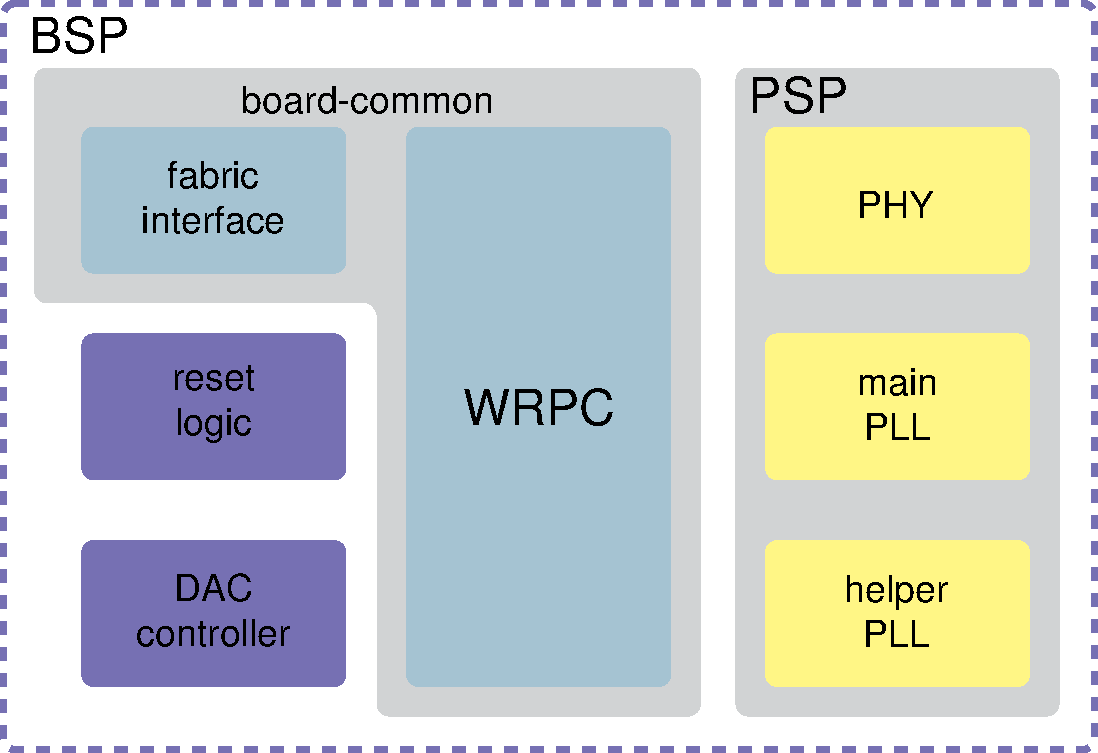
\includegraphics[width=.6\textwidth]{fig/wrpc_board.pdf}
    \caption{WRPC HDL abstraction hierarchy}
    \label{fig:wrpc_board}
  \end{center}
\end{figure}

The WRPC provides several levels of abstractions and VHDL modules, depending on the target
system. These are presented in Figure~\ref{fig:wrpc_board}. At the highest level of abstraction, the
WRPC provides Board Support Packages (BSPs), available for all officially supported boards. All BSP
modules share a common part (the ``board-common'' module) which encapsulates the WRPC core itself,
together with a selection of interfaces for connecting the core the the user FPGA
logic. Furthermore, each BSP also makes use of a Platform Support Package (PSP), which groups
together and instantiates all the FPGA-specific parts (typically hard IP provided by the FPGA
vendor), such as PHY, PLLs and clock buffers.

Thus, depending on the users' systems and needs, several scenarios might be available for
instantiating the WRPC into their designs.

\begin{description}
  \item[Option 1: Supported board.] In this simplest of scenarios, it will be enough to just
    instantiate the provided BSP into the users' designs and configure it via the provided generics.
  \item[Option 2: Supported FPGA platform.] The users could draw inspiration from an existing BSP
    based on the same platform, reusing the board-common module and PSP, while adapting the parts
    that are unique to their designs.
  \item[Option 3: Unsupported FPGA platform.] There is significant work involved in this
    scenario. In addition to providing the details for their board (just like for option 2), users
    also have to write their own PSP. It should be possible though to reuse the board-common
    module. Furthermore, if the unsupported platform is related to a supported one, it could be that
    the PHY and/or PLLs will also be reused, perhaps with minor adjustments.
\end{description}

When writing a new BSP or PSP, it's worth discussing it first in the
\href{http://www.ohwr.org/mailing_list/show?project_id=white-rabbit}{white-rabbit-dev} mailing
list. Perhaps there is already some preliminary support underway. It's also worth considering
sharing your work so that it can be merged with the project and added to the list of supported
platforms/boards.

The rest of this section describes the various modules in more detail. The WRPC module is presented
in Section~\ref{sec:hdl_wrpc}. The platform support modules are presented in
Section~\ref{sec:hdl_platform}, while the board support modules are presented in
Section~\ref{sec:hdl_board}.



\newpage
\section{Possible Errors}
\label{sec:failures}
This section tries to identify all the possible ways the White Rabbit PTP Core can
fail. The structure of each error description is the following:
\begin{itemize}[leftmargin=0pt]
	\item [] \underline{Severity}: describes how critical is the fault. Currently
		we distinguish two severity levels:
		\begin{packed_items}
			\item WARNING - means that despite the fault the synchronization
				functionality was not affected so the WRPC behaves correctly in the WR
				network.
			\item ERROR - means that the fault is critical and most probably a WRPC
				misbehaves.
		\end{packed_items}
	\item [] \underline{Mode}: for timing failures, it describes which modes are
		affected. Possible values are:
		\begin{packed_items}
			\item \emph{Slave} - the WR PTP Core synchronizes to another WR device.
			\item \emph{Grand Master} - the WR node (WR PTP Core) at the top of the
				synchronization hierarchy. It is synchronized to an external clock (e.g.
				GPS, Cesium) and provides timing to other WR/PTP devices.
			\item \emph{Master} - the WR node (WR PTP Core) at the top of the
				synchronization hierarchy. It provides timing to other WR/PTP devices
				but runs from a local oscillator (not synchronized to an external
				clock).
			\item \emph{all} - any WR PTP Core can be affected regardless the timing
				mode.
		\end{packed_items}

	\item [] \underline{Description}: What the problem is about, how important it
		is and what are the effects if it occurs.
	\item [] \underline{SNMP objects}: Which SNMP objects should be monitored to
		detect the failure. These are objects from the \texttt{WR-WRPC-MIB}.
	\item [] \underline{Error/Warning condition}: condition that should be checked
		at the SNMP manager's side to detect given problem.
  \item [] \underline{Action}: list of actions that should be performed in case
    given error/warning is reported. There are some common remarks that apply to
    all situations:
    \begin{itemize}
    \item If a procedure given for a specific SNMP object does not solve the
      problem, please contact WR experts to perform a more in-depth analysis of
      the network. For this, you should provide a complete dump of the WRPC
      status generated in the first step of each procedure.
    \item The first action in most of the procedures below named Dump state
      requires simply calling a tool provided by WR developers that reads all
      the detailed information from the node and writes it to a single file
      that can be later analyzed by the experts.
    \item If a problem solving procedure requires restarting or replacing a WR
      Node working in the \emph{Grand Master} mode, please make sure that after
      the repair, all other WR devices in the network are synchronized and do
      not report any problems.
    \item If a procedure requires replacing a WR ndoe with a new unit, the
      broken one should be handled to WR experts or the switch manufacturer to
      investigate the problem.
    \end{itemize}
\end{itemize}

\subsection{Timing error}
\label{sec:timing_fail}
As a timing error we define the WR PTP Core not being able to synchronize its
local time to the WR Master (if WRPC runs in the slave mode), or not being able
to provide correct WR time to the rest of the WR network (if WRPC runs in the
master mode).

\noindent This section contains the list of faults leading to a timing error.

\subsubsection{\bf PTP/PPSi went out of \texttt{TRACK\_PHASE}}
		\label{fail:timing:ppsi_track_phase}
		\begin{pck_descr}
			\item [] \underline{Severity}: ERROR
			\item [] \underline{Mode}: \emph{Slave}
			\item [] \underline{Description}:\\
				If the \emph{PTP/PPSi} WR servo goes out of the \texttt{TRACK\_PHASE}
				state, this means something bad has happened and the node lost the
				synchronization to its Master.
			\item [] \underline{SNMP objects}:\\
				{\footnotesize
				\snmpadd{WR-WRPC-MIB::wrpcPtpServoStateN}\\
				\snmpadd{WR-WRPC-MIB::wrpcPtpServoStateErrCnt} }
			\item [] \underline{Error condition}:\\
				{\footnotesize
				\texttt{wrpcPtpServoStateErrCnt != wrpcPtpServoStateErrCnt\_prev} }
      \item [] \underline{Action}:
        \begin{pck_proc}
        \item Dump state
        \item Check the status of the WR Master - timing source. In case it has
          reported some problems, please follow the diagnostics document for the
          WR Switch.
        \item If the Switch did not report any problems, restart the WR Node.
        \item If the problem persists replace the WR Node hardware with a new
          unit.
        \item If the problem persists, please notify WR experts.
        \end{pck_proc}
		\end{pck_descr}

\subsubsection{\bf Offset jump not compensated by Slave}
		\label{fail:timing:offset_jump}
		\begin{pck_descr}
			\item [] \underline{Severity}: ERROR
			\item [] \underline{Mode}: \emph{Slave}
			\item [] \underline{Description}:\\
				This may happen if the Master resets its WR time counters (e.g. because
				it lost the link to its Master higher in the hierarchy or to external
				clock), but the WR Slave does not follow the jump.
				\item [] \underline{SNMP objects}:\\
				{\footnotesize
				\snmpadd{WR-WRPC-MIB::wrpcPtpClockOffsetPsHR}\\
				\snmpadd{WR-WRPC-MIB::wrpcPtpClockOffsetErrCnt} }
			\item [] \underline{Error condition}:\\
				{\footnotesize
				\texttt{wrpcPtpClockOffsetErrCnt != wrpcPtpClockOffsetErrCnt\_prev} }
      \item [] \underline{Action}:
        \begin{pck_proc}
        \item Dump state
        \item Check the status of the WR Master - timing source. Normally the
          time jumps should not happen and if they do, the problem should be
          investigated on the WR Master side (e.g. \emph{Grand Master} unlocked
          from the external reference).
        \item Restart the WR Node and let it synchronize again.
        \end{pck_proc}
		\end{pck_descr}

\subsubsection{\bf Detected jump in the RTT value calculated by \emph{PTP/PPSi}}
		\label{fail:timing:rtt_jump}
		\begin{pck_descr}
			\item [] \underline{Severity}: ERROR
			\item [] \underline{Mode}: \emph{Slave}
			\item [] \underline{Description}:\\
				Once a WR link is established the round-trip delay (RTT) can change
				smoothly due to the temperature variations. However, if a sudden jump is
				detected, that means that an erroneous timestamp was generated either on
				the Master or the Slave side.
				One cause of that could be the wrong value of the t24p transition point.
			\item [] \underline{SNMP objects}:\\
				{\footnotesize
				\snmpadd{WR-WRPC-MIB::wrpcPtpRTT}\\
				\snmpadd{WR-WRPC-MIB::wrpcPtpRTTErrCnt} }
			\item [] \underline{Error condition}:\\
				{\footnotesize
				\texttt{wrpcPtpRTTErrCnt != wrpcPtpRTTErrCnt\_prev} }
      \item [] \underline{Action}:
        \begin{pck_proc}
        \item Dump state.
        \item Check the status status of the WR Master - timing source.
          Eventually proceed to investigate the problem on the WR Master side.
        \item Restart the Node.
        \item If the problem persists, replace the WR Node with a new unit.
        \end{pck_proc}
		\end{pck_descr}

\subsubsection{\bf Wrong $\Delta_{TXM}$, $\Delta_{RXM}$, $\Delta_{TXS}$,
		$\Delta_{RXS}$, $\alpha$ values are reported to the \emph{PTP/PPSi} daemon}
		\label{fail:timing:deltas_report}
		\begin{pck_descr}
			\item [] \underline{Severity}: ERROR
			\item [] \underline{Mode}: \emph{Slave}
			\item [] \underline{Description}:\\
				If \emph{PTP/PPSi} doesn't get the correct values of fixed hardware delays,
				it won't be able to calculate a proper Master-to-Slave delay. Although
				the estimated offset in \emph{PTP/PPSi} is close to 0, the WRS won't be
				synchronized to the Master with the sub-nanosecond accuracy.
			\item [] \underline{SNMP objects}:\\
				{\footnotesize
				\snmpadd{WR-WRPC-MIB::wrpcPtpDeltaTxM}\\
				\snmpadd{WR-WRPC-MIB::wrpcPtpDeltaRxM}\\
				\snmpadd{WR-WRPC-MIB::wrpcPtpDeltaTxS}\\
				\snmpadd{WR-WRPC-MIB::wrpcPtpDeltaRxS}\\
				\snmpadd{WR-WRPC-MIB::wrpcPtpAlpha} }
			\item [] \underline{Error condition}:\\
				{\footnotesize
				\texttt{wrpcPtpDeltaTxM == 0 || wrpcPtpDeltaRxM == 0 ||}\\
				\texttt{wrpcPtpDeltaTxS == 0 || wrpcPtpDeltaRxS == 0 ||}\\
				\texttt{wrpcPtpAlpha == 0} }
      \item [] \underline{Action}:
        \begin{pck_proc}
        \item Check if the correct calibration values are entered both for the WR
          Node and WR Master. WR Switch will report this in its own SNMP status
          objects.
        \item Check the White Rabbit PTP Core User Manual
          \footnote{\url{http://www.ohwr.org/projects/wr-cores/wiki/Current\_release}}
          for the instructions how the calibration values can be configured
          locally or remotely using SNMP SET objects.
        \end{pck_proc}
		\end{pck_descr}

\subsubsection{\bf PTP servo is not updating}
		\label{fail:timing:servo_not_updating}
		\begin{pck_descr}
			\item [] \underline{Severity}: ERROR
			\item [] \underline{Mode}: \emph{Slave}
			\item [] \underline{Description}:\\
				If PTP servo is not updating, we still increment the internal timing
				counters, but don't have updated information on the Master time and link
				delay. After some time the slave local time will drift away from the
				master.
			\item [] \underline{SNMP objects}:\\
				{\footnotesize
				\snmpadd{WR-WRPC-MIB::wrpcPtpServoUpdates}\\
				\snmpadd{WR-WRPC-MIB::wrpcPtpServoUpdateTime} }
			\item [] \underline{Error condition}:\\
				{\footnotesize
				\texttt{wrpcPtpServoUpdates != wrpcPtpServoUpdates} }
      \item [] \underline{Action}:
        \begin{pck_proc}
        \item Dump state
        \item Check if the PTP frames are flowing between the WR Node and its
          timing master (error \ref{fail:timing:no_frames}).
        \item Check the status of the WR Master - timing source.
        \item Check if the SoftPLL did not unlock (error
          \ref{fail:timing:spll_unlock}).
        \item Restart the WR Node.
        \item If the problem persists, replace the WR Node with a new unit.
        \end{pck_proc}
		\end{pck_descr}

\subsubsection{\bf \emph{SoftPLL} became unlocked}
		\label{fail:timing:spll_unlock}
		\begin{pck_descr}
			\item [] \underline{Severity}: ERROR / WARNING
			\item [] \underline{Mode}: \emph{all}
			\item [] \underline{Description}:\\
				If the \emph{SoftPLL} loses lock, for any reason, Slave, Master or Grand
				Master node can no longer be syntonized and phase aligned with its time
				source. WRPC in Master mode without properly locked Helper PLL is not
				able to perform reliable phase measurements for enhancing Rx timestamps
				resolution. For a Grand Master the reason of \emph{SoftPLL} going out of
				lock might be disconnected 1-PPS/10MHz signals or that the external
				clock is down.
			\item [] \underline{SNMP objects}:\\
				{\footnotesize
				\snmpadd{WR-WRPC-MIB::wrpcSpllMode}\\
				\snmpadd{WR-WRPC-MIB::wrpcSpllSeqState}\\
				\snmpadd{WR-WRPC-MIB::wrpcSpllAlignState}\\
				\snmpadd{WR-WRPC-MIB::wrpcSpllHlock}\\
				\snmpadd{WR-WRPC-MIB::wrpcSpllMlock}\\
				\snmpadd{WR-WRPC-MIB::wrpcSpllDelCnt} }
			\item [] \underline{Error condition}:\\
				{\footnotesize
        \texttt{wrpcSpllSeqState != ready\emph{(3)} ||}\\
        \texttt{[wrpcSpllMode == grandmaster\emph(1) \&\& wrpcAlignState != locked\emph{(6)}] ||}\\ % GrandMaster not locked
        \texttt{[wrpcSpllMode == slave\emph{(3)} \&\& wrpcSpllHlock == 0] ||}\\ % Spll slave and Hpll unlocked
				\texttt{[wrpcSpllMode == slave\emph{(3)} \&\& wrpcSpllMlock == 0] ||}\\ % Spll slave and Mpll unlocked
        \texttt{[wrpcSpllMode != grandmaster\emph{(1)} \&\& wrpcSpllMode != master\emph{(2)} \&\& wrpcSpllMode != slave\emph{(3)}]}} % Spll in neither of the GM/Master/Slave modes
			\item [] \underline{Warning condition}:\\
				{\footnotesize
        \texttt{[wrpcSpllMode == grandmaster\emph{(1)} \&\& wrpcSpllDelCnt > 0]}} % GrandMaster has unlocked from reference at some point
      \item [] \underline{Action for \emph{Grand Master} WR Node}:
        \begin{pck_proc}
        \item Dump state
        \item Check 1-PPS and 10MHz signals coming from an external source.
          Verify if they are properly connected and, in case of a GPS receiver,
          check if it is synchronized and locked.
        \item Restart the WR Node
        \item If the problem persists, replace the WR Node with a new unit
        \end{pck_proc}
      \item [] \underline{Action for \emph{Slave} WR Node}:
        \begin{pck_proc}
        \item Dump state
        \item Check the status of the WR Master - timing source. Eventually
          proceed to investigate the problem on the Master.
        \item Verify if the WR link was not lost and re-initialized by checking
          the SNMP manager software logs.
        \item Restart the WR Node
        \item If the problem persists, replace the WR Node with a new unit.
        \end{pck_proc}
		\end{pck_descr}

\subsubsection{\bf PTP frames don't reach LM32}
		\label{fail:timing:no_frames}
		\begin{pck_descr}
			\item [] \underline{Severity}: ERROR
			\item [] \underline{Mode}: \emph{all}
			\item [] \underline{Description}:\\
				In this case, \emph{PTP/PPSi} will fail to stay synchronized and provide
				synchronization. Even if the WR servo is in the \texttt{TRACK\_PHASE}
				state, it calculates a new phase shift based on the Master-to-Slave delay
				variations. To calculate these variations, it still needs timestamped
				PTP frames flowing. There could be several causes of such fault:
				\begin{itemize}
          \item WR Switch problem
					\item wrong VLANs configuration
					\item WR PTP Core HDL problem
				\end{itemize}
			\item [] \underline{SNMP objects}:\\
				{\footnotesize
				\snmpadd{WR-WRPC-MIB::wrpcPtpTx}\\
				\snmpadd{WR-WRPC-MIB::wrpcPtpRx}\\
				\snmpadd{WR-WRPC-MIB::wrpcPortInternalTx}\\
				\snmpadd{WR-WRPC-MIB::wrpcPortInternalRx} }
			\item [] \underline{Error condition}:\\
				{\footnotesize
				\texttt{wrpcPtpTx == wrpcPtpTx\_prev || wrpcPtpRx == wrpcPtpRx\_prev ||}\\
				\texttt{wrpcPortInternalTx == wrpcPortInternalTx\_prev ||}\\
				\texttt{wrpcPortInternalRx == wrpcPortInternalRx\_prev} }
      \item [] \underline{Action}:
        \begin{pck_proc}
        \item Dump state.
        \item Check the status of the WR Master - timing source. Especially if
          the PTP daemon is still running there.
        \item Check if the VLANs configuration on the WR Node matches the
          configuration of the WR Switch where this node is connected. Wrong
          configuration (e.g. different VIDs) will cause the frames to be
          dropped.
        \item Restart the WR Node.
        \item If possible, stop or reduce any additional (heavy) traffic that
          might be sent through the WR network.
        \item If the problem persists, please notify WR experts.
        \end{pck_proc}
		\end{pck_descr}

\subsubsection{\bf Detected SFP not supported for WR timing}
		\label{fail:timing:wrong_sfp}
		\begin{pck_descr}
			\item [] \underline{Severity}: ERROR
			\item [] \underline{Mode}: \emph{all}
			\item [] \underline{Description}:\\
				By not supported SFP for WR timing we mean a transceiver that doesn't
				have the \emph{alpha} parameter and fixed hardware delays defined in the
				SFP database. The consequence is \emph{PTP/PPSi} not having the right
				values to estimate link asymmetry. Despite \emph{PTP/PPSi} offset being
				close to 0 \emph{ps}, the device won't be properly synchronized.
			\item [] \underline{SNMP objects}:\\
				{\footnotesize
				\snmpadd{WR-WRPC-MIB::wrpcPortSfpPn}\\
				\snmpadd{WR-WRPC-MIB::wrpcPortSfpInDB} }
			\item [] \underline{Error condition}:\\
				{\footnotesize
        \texttt{wrpcPortSfpInDB != inDataBase\emph{(2)}} }
      \item [] \underline{Action}:
        \begin{pck_proc}
        \item Check if the SFP database is correctly defined by making sure if
          error \ref{fail:timing:no_sfpdb} is not reported.
        \item Change the optical SFP transceiver in the WR Node. Either it is
          broken and its ID cannot be read correctly, or a non-supported
          transceiver was plugged to the device.
        \end{pck_proc}
		\end{pck_descr}

\subsubsection{\bf SFP database not configured}
		\label{fail:timing:no_sfpdb}
		\begin{pck_descr}
			\item [] \underline{Severity}: ERROR
			\item [] \underline{Mode}: \emph{all}
			\item [] \underline{Description}:\\
				If there are no SFP entries in the database, any (even WR-supported) SFP
				cannot be matched with the calibration values for a given hardware and
				fiber. Despite \emph{PTP/PPSi} offset being close to 0 \emph{ps}, the
				device won't be properly synchronized.
			\item [] \underline{SNMP objects}:\\
				{\footnotesize
				\snmpadd{WR-WRPC-MIB::wrpcSfpDeltaTx.<n>}\\
				\snmpadd{WR-WRPC-MIB::wrpcSfpDeltaRx.<n>} }
			\item [] \underline{Note}: It's enough to try reading index 1 of the above
				SNMP objects tables to make sure there is at least one entry in the
				database.
			\item [] \underline{Error condition}:\\
				{\footnotesize
				Error when trying to get \texttt{wrpcSfpDeltaTx.1} and \texttt{wrpcSfpDeltaRx.1} SNMP objects}
      \item [] \underline{Action}:
        \begin{pck_proc}
        \item Check the White Rabbit PTP Core User
          Manual\footnote{\url{http://www.ohwr.org/projects/wr-cores/wiki/Current\_release}}
          for the instructions how the calibration values can be configured
          locally or remotely using SNMP SET objects.
        \end{pck_proc}
		\end{pck_descr}

\newpage
\subsection{Other errors}
\label{sec:other_fail}

\subsubsection{\bf WR link is down or FPGA not programmed or FPGA programmed with incorrect bitstream}
		\label{fail:timing:master_down}
		\begin{pck_descr}
			\item [] \underline{Severity}: ERROR
			\item [] \underline{Mode}: \emph{all}
			\item [] \underline{Description}:\\
				We monitor the WRPC over the WR network. We can realize if this only
				communication link is down by either SNMP requests timeouts or
				periodically pinging the device.
			\item [] \underline{SNMP objects}: \emph{(none)}
			\item [] \underline{Error condition}:\\
				{\footnotesize
				SNMP request timeout or PING timeout}
      \item [] \underline{Action}:
        \begin{pck_proc}
        \item Investigate on the computer/front-end where the WR Node card is
          installed, if all the drivers are properly loaded and if the FPGA gets
          programmed. You can take another WR Master device and connect it
          locally to verify if the WR Node is programmed correctly.
        \item Check the fiber link e.g. by connecting another WR Node, with a
          different SFP transceiver to the same fiber.
        \item If there is still no link on the new WR Node, try on the Master
          side connecting the fiber to another port of the WR Switch (using
          different SFP transceiver).
        \item If there is still no link, the fiber connection is either dirty or
          broken.
        \end{pck_proc}
		\end{pck_descr}


\subsubsection{\bf WR PTP Core reset}
		\label{fail:other:reset}
		\begin{pck_descr}
			\item [] \underline{Severity}: ERROR
			\item [] \underline{Description}:\\
				If the WRPC was reset it might either mean that there was a power cut or
				some not yet known bug caused the WRPC software to crash.
			\item [] \underline{SNMP objects}:\\
				{\footnotesize
				\snmpadd{WR-WRPC-MIB::wrpcTimeSystemUptime} }
			\item [] \underline{Error condition}:\\
				{\footnotesize
				\texttt{wrpcTimeSystemUpdate < wrpcTimeSystemUpdate\_prev} }
      \item [] \underline{Action}:
        \begin{pck_proc}
        \item Dump state.
        \item Check if there was a power cut e.g. by checking the uptime of the
          computer/front-end where the WR Node card is installed.
        \item If there was no power cut or intended machine restart, make a full
          state dump and report problem to WR experts.
        \end{pck_proc}
		\end{pck_descr}

\subsubsection{\bf WR PTP Core time reset}
		\label{fail:other:time_reset}
		\begin{pck_descr}
			\item [] \underline{Severity}: ERROR
			\item [] \underline{Description}:\\
				If the WRPC internal time counters are reset, this might mean the WR
				Master in the network has some problems and WRPC has followed the time
				reset. If that's not the case, this might mean some not yet known bug
				caused the WRPC time reset.
			\item [] \underline{SNMP objects}:\\
				{\footnotesize
				\snmpadd{WR-WRPC-MIB::wrpcTimeTAI}\\
				\snmpadd{WR-WRPC-MIB::wrpcTimeTAIString} }
			\item [] \underline{Error condition}:\\
				{\footnotesize
				\texttt{wrpcTimeTAI == 0} }
      \item [] \underline{Action}:
        \begin{pck_proc}
        \item Dump state.
        \item Check the status of the WR Master - timing source.
        \item Check in the SNMP manager software logs, if there were no
          \emph{link down} errors for the WR Node or the WR Master Switch. In
          that case, the SFP optical transceivers should be changed or the fiber
          link should be investigated.
        \end{pck_proc}
		\end{pck_descr}

\subsubsection{\bf Temperature of the node too high}
		\label{fail:other:temp}
		\begin{pck_descr}
			\item [] \underline{Severity}: WARNING
			\item [] \underline{Description}:\\
				If the temperature raises too high we might break our electronics. It
				also means that most probably something is wrong with the node cooling.
			\item [] \underline{SNMP objects}:\\
				{\footnotesize
				\snmpadd{WR-WRPC-MIB::wrpcTemperatureName.<n>}\\
				\snmpadd{WR-WRPC-MIB::wrpcTemperatureValue.<n>} }
			\item [] \underline{Error condition}:\\
				{\footnotesize
				\texttt{wrpcTemperatureValue.<n> > THRESHOLD} }
      \item [] \underline{Action}:
        \begin{pck_proc}
        \item Check the cooling for the computer/front-end/rack where the WR
          Node is installed.
        \end{pck_proc}
		\end{pck_descr}

\newpage
\section{List of exported SNMP objects}
This section lists all the SNMP objects exported by the WR PTP Core. The objects
provide read-only values unless stated otherwise in their description.\\

\printnoidxglossary[type=snmp_status,title=,style=objtree,sort=def]


% add not used entries, but don't display their's section
% based on:
% http://tex.stackexchange.com/questions/115635/glossaries-suppress-pages-when-using-glsaddall
\forallglsentries{\thislabel}%
{%
  \ifglsused{\thislabel}{}{\glsadd[format=ignore]{\thislabel}}%
}

\end{document}
